\documentclass{article}

\pdfminorversion=5 % erlaubt das Einfügen von pdf-Dateien bis Version 1.7, ohne eine Fehlermeldung zu werfen (keine Garantie für fehlerfreies Einbetten!)
\usepackage[utf8]{inputenc} % muss als erstes eingebunden werden, da Meta/Packages ggfs. Sonderzeichen enthalten

\newcommand{\titel}{Entwicklung einer allgemeinen Ressourcenverwaltung}
\newcommand{\untertitel}{für Diagnostikgeräte via gRPC}
\newcommand{\kompletterTitel}{\titel{} \untertitel}

\newcommand{\autorName}{Lukas Klettke}
\newcommand{\autorAnschrift}{Am Mühlenteich 17}
\newcommand{\autorOrt}{23611 Bad Schwartau}
\newcommand{\autorPfnr}{Prüflingsnummer: 0000826104}

\newcommand{\betriebLogo}{LogoBetrieb.jpg}
\newcommand{\betriebName}{\textsc{EUROIMMUN} Medizinische Labordiagnostika AG}
\newcommand{\betriebNameKzf}{\textsc{EUROIMMUN}}
\newcommand{\mutterBetriebName}{\textsc{PerkinElmer} Inc.}
\newcommand{\betriebAnschrift}{Am Seekamp 31}
\newcommand{\betriebOrt}{23560 Lübeck}

\newcommand{\ausbildungsberuf}{Fachinformatiker für Anwendungsentwicklung}
\newcommand{\betreff}{Dokumentation zur betrieblichen Projektarbeit}
\newcommand{\pruefungstermin}{Winter 2021}
\newcommand{\abgabeOrt}{Lübeck}
\newcommand{\abgabeTermin}{01.12.2021}
 % Metadaten zu diesem Dokument (Autor usw.)
% Anpassung an Landessprache ---------------------------------------------------
\usepackage[ngerman]{babel}

% Umlaute ----------------------------------------------------------------------
%   Umlaute/Sonderzeichen wie äüöß direkt im Quelltext verwenden (CodePage).
%   Erlaubt automatische Trennung von Worten mit Umlauten.
% ------------------------------------------------------------------------------
\usepackage[T1]{fontenc}
\usepackage{textcomp} % Euro-Zeichen etc.

% Schrift ----------------------------------------------------------------------
\usepackage[pdfspacing]{classicthesis}
\usepackage{lmodern} % bessere Fonts
\usepackage{relsize} % Schriftgröße relativ festlegen

% Tabellen ---------------------------------------------------------------------
\usepackage{xcolor}
\usepackage{colortbl}
\usepackage{tabularx}
% für lange Tabellen
\usepackage{longtable}
\usepackage{array}
\usepackage{ragged2e}
\usepackage{lscape}

% Einfache Definition der Zeilenabstände und Seitenränder etc.
\usepackage{setspace}
\usepackage{geometry}

% Grafiken ---------------------------------------------------------------------
\usepackage[dvips,final]{graphicx} % Einbinden von JPG-Grafiken ermöglichen
\usepackage{smartdiagram}
\usepackage{graphics} % keepaspectratio
\usepackage{graphicx}
\usepackage{floatflt} % zum Umfließen von Bildern
\graphicspath{{Bilder/}} % hier liegen die Bilder des Dokuments

% Sonstiges --------------------------------------------------------------------
\usepackage[titles]{tocloft} % Inhaltsverzeichnis DIN 5008 gerecht einrücken
\usepackage{amsmath,amsfonts} % Befehle aus AMSTeX für mathematische Symbole
\usepackage{enumitem} % anpassbare Enumerates/Itemizes
\usepackage{xspace} % sorgt dafür, dass Leerzeichen hinter parameterlosen Makros nicht als Makroendezeichen interpretiert werden

\usepackage{makeidx} % für Index-Ausgabe mit \printindex
\usepackage[printonlyused]{acronym} % es werden nur benutzte Definitionen aufgelistet
\usepackage{nomencl}

% zum Einbinden von Programmcode -----------------------------------------------
\usepackage{listings}
\usepackage{hyperref} %For adding hyperlinks

\definecolor{hellgelb}{rgb}{1,1,0.9}
\definecolor{colKeys}{rgb}{0,0,1}
\definecolor{colIdentifier}{rgb}{0,0,0}
\definecolor{colComments}{rgb}{0,0.5,0}
\definecolor{colString}{rgb}{1,0,0}
\lstset{
	float=hbp,
	basicstyle=\footnotesize,
	identifierstyle=\color{colIdentifier},
	keywordstyle=\color{colKeys},
	stringstyle=\color{colString},
	commentstyle=\color{colComments},
	backgroundcolor=\color{hellgelb},
	columns=flexible,
	tabsize=2,
	frame=single,
	extendedchars=true,
	showspaces=false,
	showstringspaces=false,
	numbers=left,
	numberstyle=\tiny,
	breaklines=true,
	breakautoindent=true,
	captionpos=b,
}
\lstdefinelanguage{cs}{
	sensitive=false,
	morecomment=[l]{//},
	morecomment=[s]{/*}{*/},
	morestring=[b]",
	morekeywords={
		abstract,event,new,struct,as,explicit,null,switch
		base,extern,object,this,bool,false,operator,throw,
		break,finally,out,true,byte,fixed,override,try,
		case,float,params,typeof,catch,for,private,uint,
		char,foreach,protected,ulong,checked,goto,public,unchecked,
		class,if,readonly,unsafe,const,implicit,ref,ushort,
		continue,in,return,using,decimal,int,sbyte,virtual,
		default,interface,sealed,volatile,delegate,internal,short,void,
		do,is,sizeof,while,double,lock,stackalloc,
		else,long,static,enum,namespace,string},
}
\lstdefinelanguage{natural}{
	sensitive=false,
	morecomment=[l]{/*},
	morestring=[b]",
	morestring=[b]',
	alsodigit={-,*},
	morekeywords={
		DEFINE,DATA,LOCAL,END-DEFINE,WRITE,CALLNAT,PARAMETER,USING,
		IF,NOT,END-IF,ON,*ERROR-NR,ERROR,END-ERROR,ESCAPE,ROUTINE,
		PERFORM,SUBROUTINE,END-SUBROUTINE,CONST,END-FOR,END,FOR,RESIZE,
		ARRAY,TO,BY,VALUE,RESET,COMPRESS,INTO,EQ},
}
\lstdefinelanguage{php}{
	sensitive=false,
	morecomment=[l]{/*},
	morestring=[b]",
	morestring=[b]',
	alsodigit={-,*},
	morekeywords={
		abstract,and,array,as,break,case,catch,cfunction,class,clone,const,
		continue,declare,default,do,else,elseif,enddeclare,endfor,endforeach,
		endif,endswitch,endwhile,extends,final,for,foreach,function,global,
		goto,if,implements,interface,instanceof,namespace,new,old_function,or,
		private,protected,public,static,switch,throw,try,use,var,while,xor
		die,echo,empty,exit,eval,include,include_once,isset,list,require,
		require_once,return,print,unset},
} % verwendete Packages
% !TEX root = ../Projektdokumentation.tex

% Seitenränder -----------------------------------------------------------------
\setlength{\topskip}{\ht\strutbox} % behebt Warnung von geometry
\geometry{a4paper,left=20mm,right=20mm,top=25mm,bottom=35mm}

\usepackage[
	automark, % Kapitelangaben in Kopfzeile automatisch erstellen
	headsepline=.4pt,
	plainheadsepline
]{scrlayer-scrpage}

% Kopf- und Fußzeilen ----------------------------------------------------------
\pagestyle{scrheadings}

% Kopfzeile
\renewcommand{\headfont}{\normalfont} % Schriftform der Kopfzeile
\ihead{\large{\textsc{\titel}}\\ \small{\untertitel} \\[2ex] \textit{\headmark}}
\chead{}
\ohead{\includegraphics[scale=1.05]{\betriebLogo}}
\setlength{\headheight}{10mm} % Höhe der Kopfzeile
%\setheadwidth[0pt]{textwithmarginpar} % Kopfzeile über den Text hinaus verbreitern (falls Logo den Text überdeckt)

% Fußzeile
\ifoot{\autorName}
\cfoot{}
\ofoot{\pagemark}

\newcommand{\headingSpace}{1.5cm}

\renewcommand*{\othersectionlevelsformat}[3]{
  \makebox[\headingSpace][l]{#3\autodot}
}

\cftsetindents{section}{0.0cm}{\headingSpace}
\cftsetindents{subsection}{0.0cm}{\headingSpace}
\cftsetindents{subsubsection}{0.0cm}{\headingSpace}
\cftsetindents{figure}{0.0cm}{\headingSpace}
\cftsetindents{table}{0.0cm}{\headingSpace}

\onehalfspacing % Zeilenabstand 1,5 Zeilen
\frenchspacing % erzeugt ein wenig mehr Platz hinter einem Punkt

\clubpenalty = 10000
\widowpenalty = 10000
\displaywidowpenalty = 10000

\counterwithout{footnote}{section} % Fußnoten fortlaufend durchnummerieren
\setcounter{tocdepth}{3} % im Inhaltsverzeichnis werden die Kapitel bis zum Level der subsubsection übernommen
\setcounter{secnumdepth}{3} % Kapitel bis zum Level der subsubsection werden nummeriert

% Aufzählungen anpassen
\renewcommand{\labelenumi}{\arabic{enumi}.}
\renewcommand{\labelenumii}{\arabic{enumi}.\arabic{enumii}.}
\renewcommand{\labelenumiii}{\arabic{enumi}.\arabic{enumii}.\arabic{enumiii}}

% Tabellenfärbung:
\definecolor{heading}{rgb}{0.64,0.78,0.86}
\definecolor{odd}{rgb}{0.9,0.9,0.9} % Definitionen zum Aussehen der Seiten
% !TEX root = ../Projektdokumentation.tex

% Abkürzungen, ggfs. mit korrektem Leerraum
\newcommand{\bs}{$\backslash$\xspace}
\newcommand{\bspw}{bspw.\xspace}
\newcommand{\bzw}{bzw.\xspace}
\newcommand{\ca}{ca.\xspace}
\newcommand{\dahe}{\mbox{d.\,h.}\xspace}
\newcommand{\etc}{etc.\xspace}
\newcommand{\eur}[1]{\mbox{#1\,\texteuro}\xspace}
\newcommand{\evtl}{evtl.\xspace}
\newcommand{\ggfs}{ggfs.\xspace}
\newcommand{\Ggfs}{Ggfs.\xspace}
\newcommand{\gqq}[1]{\glqq{}#1\grqq{}}
\newcommand{\inkl}{inkl.\xspace}
\newcommand{\insb}{insb.\xspace}
\newcommand{\ua}{\mbox{u.\,a.}\xspace}
\newcommand{\usw}{usw.\xspace}
\newcommand{\Vgl}{Vgl.\xspace}
\newcommand{\zB}{\mbox{z.\,B.}\xspace}

% Befehle für häufig anfallende Aufgaben
\newcommand{\Abbildung}[1]{\autoref{fig:#1}}
\newcommand{\Anhang}[1]{\appendixname{}~\ref{#1}: \nameref{#1} \vpageref{#1}}
\newcommand{\includegraphicsKeepAspectRatio}[2]{\includegraphics[width=#2\textwidth,height=#2\textheight,keepaspectratio]{#1}}
\newcommand{\Zitat}[2][\empty]{\ifthenelse{\equal{#1}{\empty}}{\citep{#2}}{\citep[#1]{#2}}}
\newcommand{\Autor}[1]{\textsc{#1}} % zum Ausgeben von Autoren
\newcommand{\itemd}[2]{\item{\textbf{#1}}\\{#2}} % erzeugt ein Listenelement mit fetter Überschrift

% fügt Tabellen aus einer TEX-Datei ein
\newcommand{\tabelle}[3] % Parameter: caption, label, file
{\begin{table}[htbp]
\centering
\singlespacing
\input{Tabellen/#3}
\caption{#1}
\label{#2}
\end{table}}

\newcommand{\tabelleAnhang}[1] % Parameter: file
{\begin{center}
\singlespacing
\input{Tabellen/#1}
\end{center}}

% einfaches Wechseln der Schrift, z.B.: \changefont{cmss}{sbc}{n}
\newcommand{\changefont}[3]{\fontfamily{#1} \fontseries{#2} \fontshape{#3} \selectfont}

% Verwendung analog zu \includegraphics
\newlength{\myx} % Variable zum Speichern der Bildbreite
\newlength{\myy} % Variable zum Speichern der Bildhöhe
\newcommand\includegraphicstotab[2][\relax]{%
% Abspeichern der Bildabmessungen
\settowidth{\myx}{\includegraphics[{#1}]{#2}}%
\settoheight{\myy}{\includegraphics[{#1}]{#2}}%
% das eigentliche Einfügen
\parbox[c][1.1\myy][c]{\myx}{%
\includegraphics[{#1}]{#2}}%
}

\definecolor{AOBlau}{rgb}{0, 0.28, 0.56}

% verschiedene Befehle um Wörter semantisch auszuzeichnen ----------------------
\newcommand{\Index}[2][\empty]{\ifthenelse{\equal{#1}{\empty}}{\index{#2}#2}{\index{#1}#2}}
\newcommand{\Fachbegriff}[2][\empty]{\ifthenelse{\equal{#1}{\empty}}{\textit{\Index{#2}}}{\textit{\Index[#1]{#2}}}}
\newcommand{\NeuerBegriff}[2][\empty]{\ifthenelse{\equal{#1}{\empty}}{\textbf{\Index{#2}}}{\textbf{\Index[#1]{#2}}}}

\newcommand{\Ausgabe}[1]{\texttt{#1}}
\newcommand{\Eingabe}[1]{\texttt{#1}}
\newcommand{\Code}[1]{\texttt{#1}}
\newcommand{\Datei}[1]{\texttt{#1}}

\newcommand{\Assembly}[1]{\textsf{#1}}
\newcommand{\Klasse}[1]{\textsf{#1}}
\newcommand{\Methode}[1]{\textsf{#1}}
\newcommand{\Attribut}[1]{\textsf{#1}}

\newcommand{\Datentyp}[1]{\textsf{#1}}
\newcommand{\XMLElement}[1]{\textsf{#1}}
\newcommand{\Webservice}[1]{\textsf{#1}}

\newcommand{\Refactoring}[1]{\Fachbegriff{#1}}
\newcommand{\CodeSmell}[1]{\Fachbegriff{#1}}
\newcommand{\Metrik}[1]{\Fachbegriff{#1}}
\newcommand{\DesignPattern}[1]{\Fachbegriff{#1}}
 % eigene allgemeine Befehle, die z.B. die Arbeit mit LaTeX erleichtern

\begin{document}

\phantomsection
\thispagestyle{plain}
\pdfbookmark[1]{Deckblatt}{deckblatt}
\begin{titlepage}
	\centering
	{\scshape\LARGE Abschlussprüfung \pruefungstermin \par}
	\vspace{1cm}
	{\scshape\LARGE \ausbildungsberuf \par}
	\vspace{1cm}
	{\scshape\Large Dokumentation zur betrieblichen Projektarbeit \par}
	\vspace{1cm}
	{\huge\bfseries\titel \par}
	{\scshape\Large \untertitel \par}
	\vspace{2cm}
	{\scshape\Large Prüfungsbewerber: \par}
	{\Large\itshape \autorName \par}
	{\Large\itshape \autorAnschrift \par}
	{\Large\itshape \autorOrt \par}
	\vfill

	% Bottom of the page
	{\large \today\par}
\end{titlepage}
\cleardoublepage

\phantomsection
\thispagestyle{empty}
\pdfbookmark[1]{Eidesstattliche Erklärung}{ihkdeckblatt}
\cleardoublepage

% Preface --------------------------------------------------------------------
\renewcommand{\contentsname}{Inhaltsverzeichnis}
\phantomsection
\pagenumbering{Roman}
\pdfbookmark[1]{Inhaltsverzeichnis}{inhalt}
\tableofcontents
\cleardoublepage

% !TEX root = Projektdokumentation.tex
 % !TEX root = ../Projektdokumentation.tex
\section{Einleitung}
\label{sec:Einleitung}

\subsection{Vorstellung der eigenen Person} 
\label{sec:eigene Person}
Mein Name ist Lukas Klettke. Ich bin am 14.01.2001 in Lübeck geboren und in Bad Schwartau aufgewachsen. Dort habe ich die Grundschule und das Leibniz Gymnasium besucht. Nach zwölf Jahren Schulzeit habe ich meinen Schulweg im Jahre 2019 mit dem Abitur abgeschlossen.

Direkt nach Abschluss der Schule habe ich im August 2019 eine Ausbildung zum Fachinformatiker für Anwendungsentwicklung begonnen und bin in der Softwareentwicklung für Diagnostikgeräte tätig.

In meiner Freizeit bin ich als ehrenamtlicher Schwimmtrainer tätig, segle und fahre Rennrad.

\subsection{Vorstellung des Ausbildungsbetriebs} 
\label{sec:Ausbildungsbetrieb}
Mein Ausbildungsbetrieb ist die {\betriebName} mit Hauptsitz in {\betriebOrt} und Zweigstellen in Groß Grönau, Selmsdorf und Dassow im Norden und Rennersdorf, Pegnitz und Bernstadt im Süden Deutschlands. Durch den Verkauf der Firma im Dezember 2017 befindet sich {\betriebNameKzf} in Besitz von {\mutterBetriebName}, einem US-amerikanischen Technologieunternehmen im Bereich der Chemie- und Medizintechnik.

{\betriebNameKzf} ist ein Hersteller für diverse medizinische Diagnostika von Autoimmun-, Infektionskrankheiten und Allergien, aber auch im Bereich der Automatisierung. Meine Ausbildung findet in Dassow in der Forschung und Entwicklung von Software zur Steuerung von Diagnostikautomaten statt.

Insgesamt hat {\betriebNameKzf} mehr als 3.200 Mitarbeiter in 17 Ländern.

\subsection{Projektauslöser} 
\label{sec:Projektauslöser}
Neben der Herstellung von medizinischen Diagnostika zur manuellen Durchführung werden Geräte zur automatisierten Durchführung dessen hergestellt und vertrieben. Diese Diagnostikautomaten arbeiten mit diversen unterschiedlichen Betriebsmitteln (z.B. Reinigungsflüssigkeit zur Reinigung der Schläuche, Probenträger etc.), welche ebenfalls von {\betriebNameKzf} an die Kunden verkauft werden.

Anhand der verbrauchten Betriebsmittel der Geräte wird die Menge, der in Zukunft benötigten, berechnet und die Preise dementsprechend auf den Kunden angepasst. Außerdem wird je nach Verbrauch der Labore die Produktions- und Lagermenge optimiert.

Derzeit werden jedoch keine Daten der Verbräuche von den Gerätesoftwares erhoben, was eine manuelle Berechnung derer zur Folge hat. Diese Berechnung wird durch Außendienstmitarbeiter durchgeführt, welche die Labore besuchen und die durchgeführten Testmengen als Maßstab nutzen. Je nach Art des Gerätebetriebs ist der Verbrauch jedoch unterschiedlich: Werden z.B. 500 Tests am Stück durchgeführt, ist das Verhalten des Geräts ein Anderes, als wenn über eine Zeit von zwei Wochen 500 Tests durchgeführt werden. Somit ist bei der Berechnung eine gewisse Ungenauigkeit vorhanden, die in Zusammenhang mit einer großen Anzahl an Kunden ebenfalls große Differenzen zwischen berechneten und reellen Verbräuchen verursacht. 

Durch eine automatisierte und genauere Berechnung mithilfe von protokollierten Ressourcenverbräuchen könnten Punkte wie Preisgestaltung, Produktionsmenge oder Lagerhaltung weiter optimiert und somit Geld eingespart bzw. Gewinn maximiert werden.

\subsection{Projektumfeld}
\label{sec:Projektumfeld}
Das Projektumfeld ist der {\betriebNameKzf} Standort in Dassow. Dort befindet sich ein Teil der Entwicklung der Diagnostikgeräte und der zugehörigen Software. 

Bei diesem Projekt handelt es sich um eine Software, die ausschließlich intern eingesetzt werden soll.

Der Entwicklungsstandard für die diversen Softwares zur Steuerung der Diagnostikgeräte ist die Programmiersprache C\# in Verbindung mit dem .NET Framework.

\subsection{Projektziel}
\label{sec:Projektziel}
Ziel des Projekts ist es eine Schnittstelle zu definieren, die unabhängig von Diagnostikgerät und der entsprechenden Software implementiert werden kann. Durch diese Schnittstelle wird definiert, in welcher Form die Verbrauchsdaten abgefragt werden.

Anhand dessen wird eine Software geschrieben, die die Ressourcenverbräuche verarbeitet, eine Gesamtberechnung durchführt und den Export einer \glqq .xlsx\grqq \xspace ermöglicht, um die nachstehende Kalkulation mittels Microsoft Excel zu gewährleisten.

Die Planung eines solchen Projekts existiert bereits mehrere Jahre und wurde von der Geschäftsführung in Auftrag gegeben. Ziel ist es Daten über die Nutzung der {\betriebNameKzf} Diagnostikgeräte zur erheben, welche zur Analyse von weiteren Optimierungmöglichkeiten dienen.

\subsection{Projektschnittstellen}
\label{sec:Projektschnittstellen}
Das Projekt stellt eine {\acs{gRPC}} Schnittstelle bereit. Diese wird mithilfe einer \glqq .proto\grqq \xspace Datei definiert. Die Schnittstelle wird auf Seite des Clients implementiert und auf Seite des Servers offen gelassen, sodass die unterschiedlichen Softwares der Diagnostikgeräte diese implementieren können und die Freiheit haben, je nach Architektur und Speicherung, die Daten bereitzustellen.

Des Weiteren wird der Export einer \glqq .xlsx\grqq \xspace Datei angeboten.
 % !TEX root = ../Projektdokumentation.tex
\section{Projektplanung}
\label{sec:Projektplanung}

\subsection{Projektphasen} 
\label{sec:Projektphasen}

Tabelle~\ref{tab:Zeitplanung} zeigt die vorgesehenen Phase des Projektes.
\tabelle{Zeitplanung}{tab:Zeitplanung}{Zeitplanung}\\ 

\subsection{Ist-Analyse} 
\label{sec:IstAnalyse}
\acs{RPC}
 % !TEX root = ../Projektdokumentation.tex
\section{Entwurfsphase}
\label{sec:Entwurfsphase}

\subsection{Zielplattform}
\label{sec:Zielplattform}
Für die 64 Bit Version von Windows 10 wird ein Prozessor mit mindestens 1 GHz Arbeitsleistung oder ein {\acs{SoC}} benötigt. Die Mindestkapazität des RAM liegt bei 2 GB, der Festplattenspeicher muss mindestens 32 GB groß sein. Die Grafikkarte muss über DirectX 9 oder höher mit einem {\acs{WDDM}} 1.0 Treiber verfügen.

\subsection{Qualitätssicherung}
\label{sec:Qualitätssicherung}
Zur Sicherung der Qualität wird die Zuverlässigkeit der Software getestet. Beide Seiten der Schnittstelle müssen zu jeder Zeit erreichbar sein und auf Anfragen reagieren bzw. Anfragen senden können. Gleichzeitig muss in Fehlerfällen reagiert werden und eine weitere Bereitstellung der Dienste gesichert sein. Zur Gewährleistung dessen wird die Software im fertigen Zustand Stresstests mit großen Datenmengen und absichtlich verursachten Fehlerfällen ausgesetzt. 

Um die Einsatzbereitschaft zu gewährleisten, ist es erforderlich, die einzubindenden Bibliotheken eindeutig zu dokumentieren um die Menge der möglichen Implementierungsfehler so klein wie möglich zu halten.
 % !TEX root = ../Projektdokumentation.tex
\section{Realisierung}
\label{sec:Realisierung}

\subsection{Eingesetzte Technologien}
\label{sec:EingesetzteTechnologien}
Für die Entwicklung der Schnittstelle, mit der die Verbräuche der Betriebsmittel der Diagnostikgeräte abgefragt werden, wird {\acs{gRPC}} verwendet. {\acs{gRPC}} ist ein Open-Source {\acs{RPC}} System, welches von Google entwickelt wird.

{\acs{RPC}} ist eine Technologie, die es möglich macht, Prozeduren auf anderen Geräte auszuführen, als auf dem, wo es aufgerufen wird (meistens innerhalb eines Netzwerks). Durch diese Auslagerung kann Datenverarbeitung auf andere Geräte ausgelagert werden, ohne dass ein Unterschied in der Entwicklung entsteht. Daraus ergibt sich eine Form der Client-Server-Architektur, bei der der aufrufende Part den Client und der ausführende Part den Server darstellt. Die Kommunikation basiert auf dem \glqq request-response\grqq \space Protokoll, welche synchron via http abläuft. Schickt der Client eine Abfrage, ist er während der Bearbeitung durch den Server blockiert\footnote{Wikipedia: \url{https://en.wikipedia.org/wiki/Remote_procedure_call} (Stand 08.11.2021 10:15 Uhr)}.

Die Wahl der Technologie fiel auf {\acs{gRPC}}, da dieses bereits in der Firma genutzt wurde und somit eine Vorgabe darstellte.

Die Anwendung wird mit C\# entwickelt. Dafür wird die Version 4.8 des .NET Frameworks verwendet.

Zum exportieren von \glqq .xlsx\grqq \space Dateien wird das {\acs{NuGet}}-Paket \glqq Microsoft.Office.Interop.Excel\grqq \space verwendet. Die Dokumentation befindet sich auf der Microsoft Docs Webseite\footnote{Microsoft.Office.Interop.Excel: \url{https://docs.microsoft.com/en-us/dotnet/api/microsoft.office.interop.excel?view=excel-pia}} des Frameworks.

Als Hilfe zur Implementierung wird {\acs{Prism}} eingesetzt. Durch die Nutzung ergibt sich eine einfach Einbindung von {\acs{IoC}}. Mithilfe von {\acs{IoC}} können Konstruktoren automatisch initialisiert werden, woraus sich eine deutlich erhöhte Übersichtlichkeit des Programmcodes ergibt.

\subsection{Entwicklungsumgebung}
\label{sec:Entwicklungsumgebung}
Zur Entwicklung wird Visual Studio Professional 2019 verwendet. Die IDE wurde durch die ReSharper Extension von Jetbrains erweitert. ReSharper fügt Tools für Refactoring und das Erkennen von Code Smells\footnote{Wikipedia: \url{https://de.wikipedia.org/wiki/Code-Smell} (Stand 10.11.2021 12:15 Uhr)} hinzu. So wird gewährleistet, dass sauberer und qualitativ hochwertiger Quellcode produziert wird.

\subsection{Erstellung einer Benutzeroberfläche}
\label{sec:ErstellungEinerBenutzeroberfläche}
Die Oberfläche wurde mit {\acs{WPF}} entworfen. Als Architekturmodell wird ein Hybrid aus zwei {\acs{MVVM}} Architekturen angewendet. Die einzelnen Bestandteile (im Folgenden \glqq Views\grqq \space genannt) verwenden je eine {\acs{MVVM}} Architektur, womit ist die Benutzeroberfläche von der Logik abgekoppelt ist. Die Werte werden mittels Data Binding in die Screens integriert. Um die einzelnen Views in der Oberfläche zu verwenden, wird über ein einzelnes ViewModel kontrolliert, welche View gerade zu sehen ist.

Für die Erstellung eines einheitlichen Designs wird die {\betriebNameKzf} interne Design Bibliothek genutzt, die nach der Material Design Sprache von Google geschrieben ist. Implementiert ist diese ebenfalls in {\acs{WPF}} und lässt sich durch Auslagerung in sogenannte \glqq Resource Dictionaries\grqq \space einbinden.

\begin{figure}[htb]
	\centering
	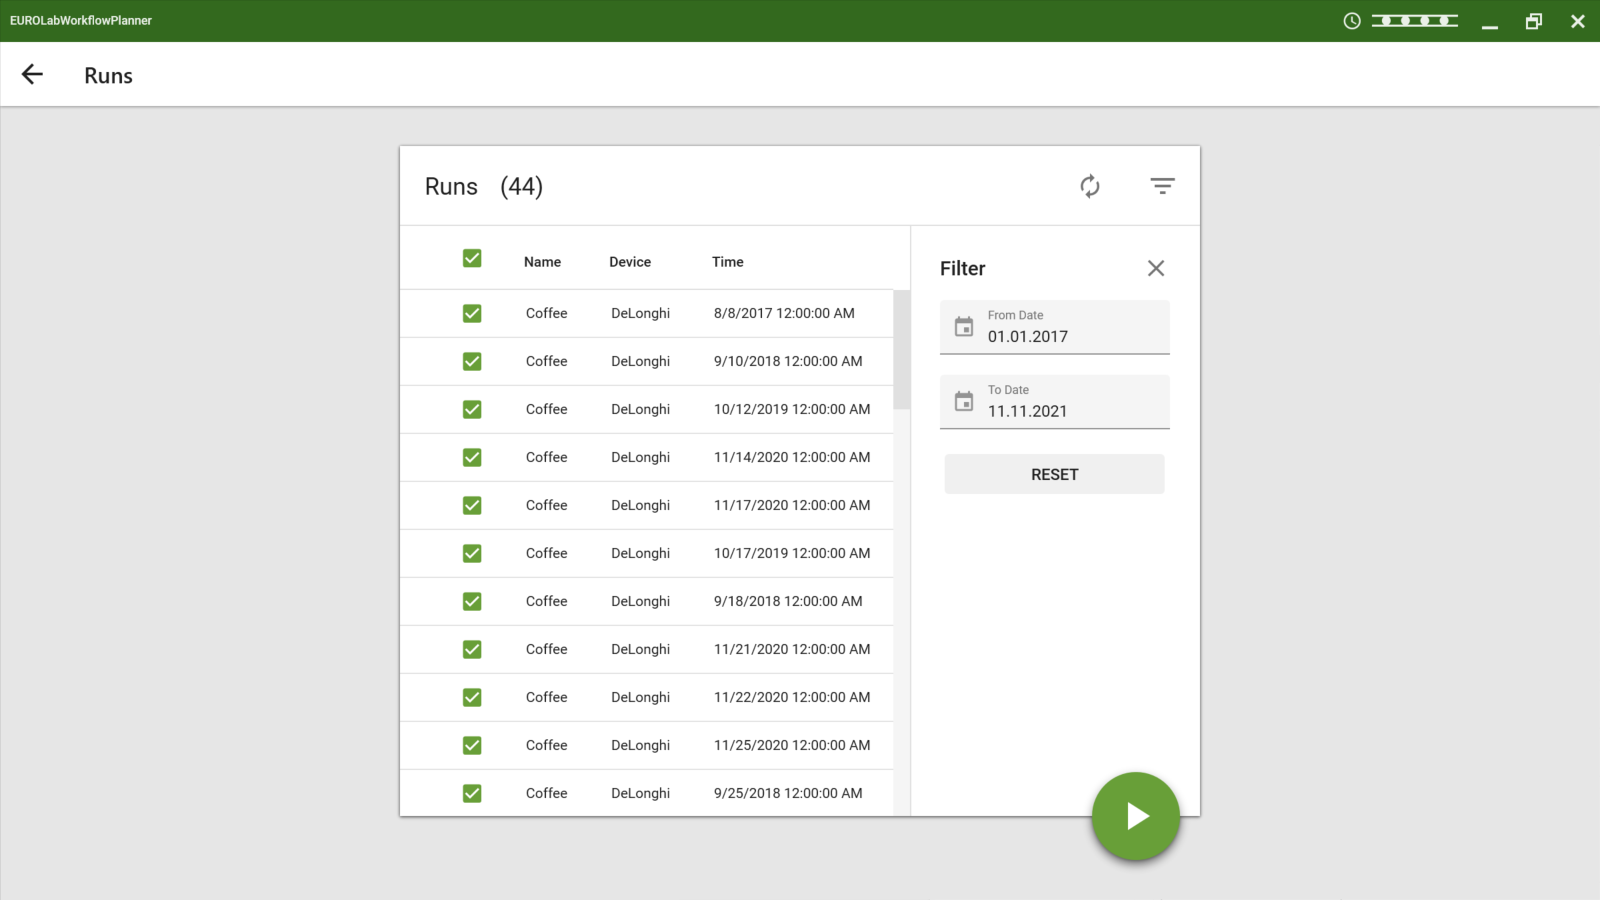
\includegraphics[scale=0.5]{Bilder/RunsAnsicht.png}
	\caption{Hauptansicht der abgefragten Daten}
	\label{fig:Runs}
\end{figure} 

\subsection{Implementierung der Geschäftslogik}
\label{sec:ImplementierungDerGeschäftslogik}
Die Implementierung der Schnittstelle via {\acs{gRPC}} wurde vom Betrieb vorgegeben, da die Technologie an anderen Stelle bereits verwendet wurde und somit ein gewisses Grundwissen vorhanden war.

Zunächst war das Ziel eine Schnittstelle zu entwickeln, die einfach von anderen Gerätesoftware-Projekten implementiert werden kann. Diese Schnittstelle wird entwickelt und in ein {\acs{NuGet}}-Paket ausgelagert. Durch die Nutzung eines Firmeninternen {\acs{GitLab}}-Servers wird dieses Paket für die firmeninterne Nutzung freigegeben.

Zur Implementierung dieser Schnittstelle muss die Klasse \glqq RPCServer\grqq \space (s. Listing~\ref{app:ServerseitigeKlasse}) initialisiert werden. In den Konstruktor wird dazu das Interface \glqq IEUROLabWorkflowPlannerService\grqq \space (s. Listing~\ref{app:Schnittstelle}) rein gereicht. Über eine eigene Implementierung des Interfaces können die Daten entsprechend der Software des Diagnostikgeräts erbracht werden.

Bei Abfrage der Daten werden Verbräuche mit Verbrauchsnamen gekennzeichnet. Anhand dieser Namen werden gleichnamige zusammengerechnet und zur besseren Übersicht gegliedert (s. Abbildung~\ref{fig:Consumptions}). Eine qualitative Bewertung der Daten findet nicht statt, die Daten werden unabhängig von Einheiten verarbeitet.

\begin{figure}[htb]
	\centering
	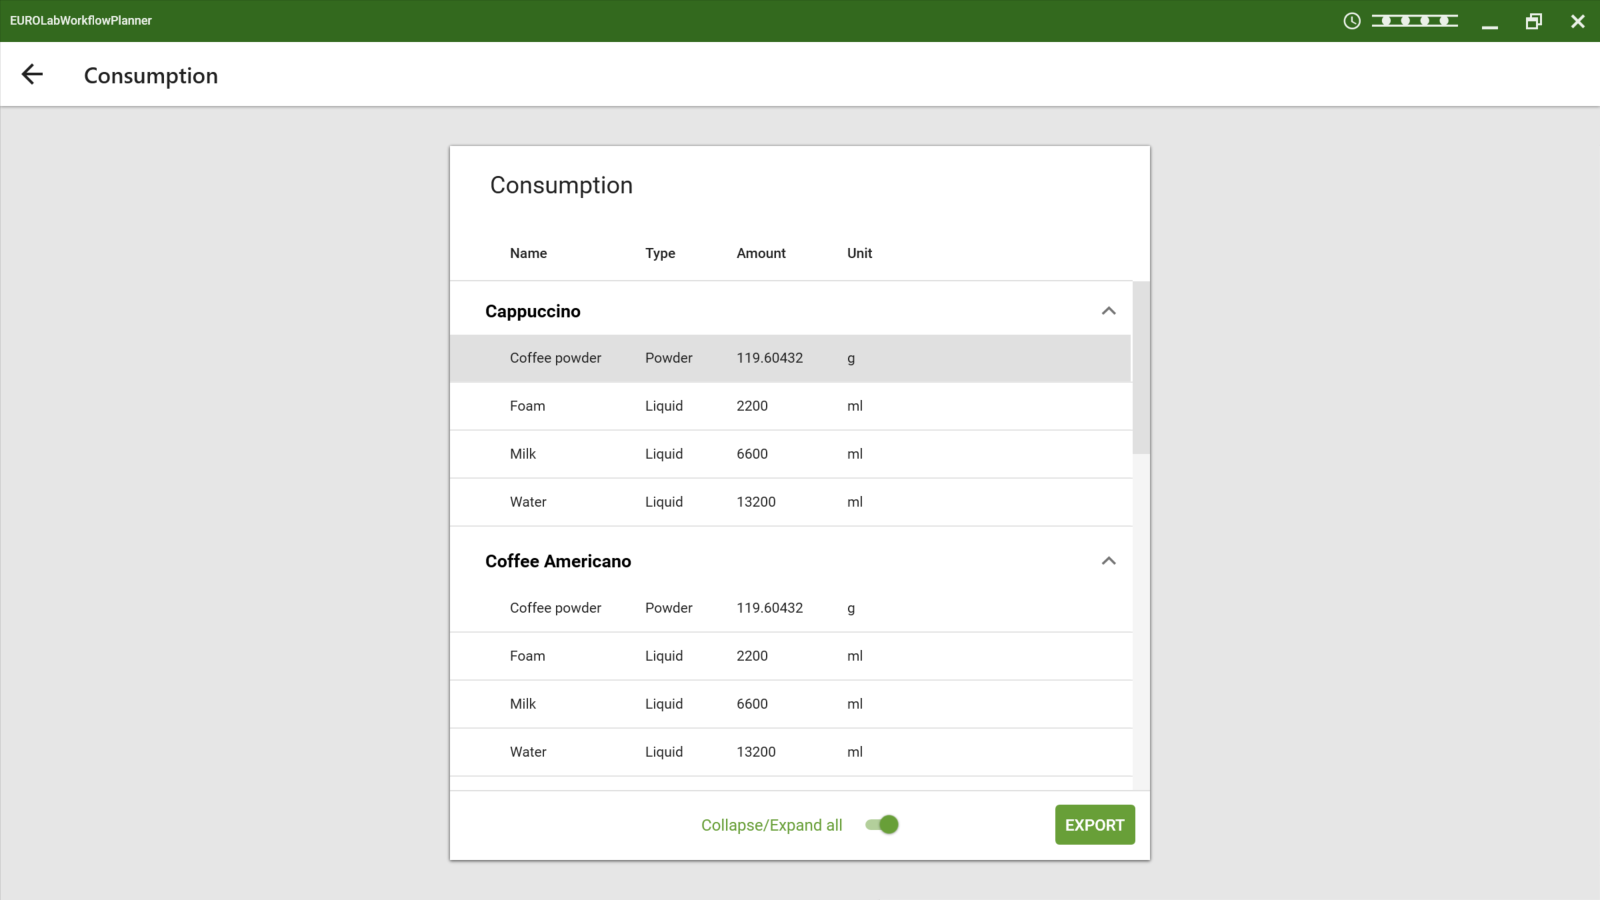
\includegraphics[scale=0.5]{Bilder/VerbrauchAnsicht.png}
	\caption{Ansicht der zusammengefassten Betriebsmittelverbräuche}
	\label{fig:Consumptions}
\end{figure}
 % !TEX root = ../Projektdokumentation.tex
\section{Abnahmephase}
\label{sec:Abnahmephase}

\subsection{Testphase}
\label{sec:Testphase}
Zur Testung der Anwendung wurden diverse Testfälle manuell durchgeführt. Da die Logik zum Großteil auf der Serverseite vorhanden ist, wurde auf Unit Tests verzichtet.

Anhand von Systemtests wurde sicher gestellt, dass alle Anforderung, die an die Software gestellt wurden umgesetzt sind. Außerdem wurde mithilfe von Performance Tests getestet, wie standhaft die Software in Punkten wie Zuverlässigkeit, Stabilität und Verfügbarkeit ist. Auch beim Senden von größeren Datenmengen von mehreren Diagnostikgeräten gleichzeitig, wies die Anwendung eine gute Performance auf und stürzte nicht ab. Ebenfalls die Serverseite funktionierte zuverlässig und war mit unterschiedlichen  Implementierungen immer erreichbar und lieferte auf Abfrage Daten.

Die Testung möglicher auftretender Fehler verlief ebenfalls ohne Mängel. Auf Fälle wie nicht erreichbare Server, Abbruch der Kommunikation oder zu große Datenmengen reagierte die Software und lief zuverlässig weiter.

\subsection{Abnahme}
\label{sec:Abnahme}
Die Abnahme der Schnittstelle und der Software erfolgt durch den Auftraggeber des Projekts, dem Anforderungsmanager zur Prüfung der Erfüllung aller Anforderungen und einem Softwaretester, der die Software ebenfalls auf Zuverlässigkeit testet.
 \input{Inhalt/Einführungsphase}
 % !TEX root = ../Projektdokumentation.tex
\section{Dokumentation}
\label{sec:Dokumentation}

\subsection{Dokumentation der Software}
\label{sec:DokumentationSoftware}
Zur Weiterentwicklung durch andere Entwickler wurde der Quellcode der Software mit Kommentaren gekennzeichnet. Neben einer kurzen Beschreibung der Klassen und Funktionen wurde darauf geachtet, dass Variablen möglichst selbsterklärend benannt sind.

Des weiteren wurde eine Anleitung zur Nutzung der Software geschrieben, die einen kurzen Überblick für den Anwender gibt.
 % !TEX root = ../Projektdokumentation.tex
\section{Abschluss}
\label{sec:Abschluss}

\subsection{Soll-/Ist-Vergleich}
\label{sec:SollIstVergleich}
Ziel des Projektes war die Erstellung und Implementierung einer Schnittstelle, die unabhängig von Diagnostikgerät Daten über Betriebsmittelverbräuche abfragen, zusammenrechnen und exportieren kann. Es wurden zwei Implementierungen der Serverseite erstellt und getestet. Es ist möglich beide Implementierungen zu nutzen. Somit wurden die Anforderungen nach einer unabhängigen Schnittstelle und einer Software, die darauf zugreift, umgesetzt und die erwarteten Funktionen bereit gestellt.

\subsection{Erweiterungsmöglichkeiten}
\label{sec:Erweiterungsmoeglichkeiten}
Durch die generische Entwicklung ist es einfach möglich anstatt einer {\acs{gRPC}} Schnittstelle eine andere Technologie einzubinden und somit sich z.B. direkt mit einer Datenbank zu verbinden oder mithilfe eines anderen Protokolls zu kommunizieren.

Anhand der frei implementierbaren Schnittstelle können weitere Projekte zur Entwicklung einer Software eines Diagnostikgeräts diese einbinden und unabhängig vom Verhalten des Geräts Daten in die vorgegebene Form bringen und zur Abfrage bereit stellen. In Zukunft könnten auf diese Weise die Abfragen der Betriebsmittelverbräuche standardisiert werden.

\subsection{Zukunft und Grenzen der Technologie}
\label{sec:ZukunftUndGrenzen}
Im Verlauf der Bearbeitung sind immer wieder Schwierigkeiten aufgetreten, die Defizite an dieser Technologie aufgewiesen haben. Beim Senden von sehr großen Datenmengen z.B. wurde die Performance der Kommunikation meist schlecht und teilweise wurden Antworten des Servers gesendet, jedoch nicht vom Client empfangen.

Gleichzeitig ist {\acs{gRPC}} im Gegensatz zu anderen ähnlichen Möglichkeiten der Netzwerk-Kommunikation nicht sehr weit verbreitet, was es schwieriger macht Entwickler zu finden, die ein gewisses Knowhow in diesem Bereich besitzen. Des weiteren ist die Kommunikation nicht standardisiert, was ebenfalls die Erweiterung und Implementierung schwieriger gestaltet. Durch die komplexe Nutzung von {\acs{HTTP2}} ist es nicht möglich {\acs{gRPC}} in den Browser zu integrieren.

Dennoch ist {\acs{gRPC}} eine gute Möglichkeit innerhalb eines lokalen Netzwerks zu kommunizieren und Daten geringer Größe zu verschicken.

\subsection{Probleme}
\label{sec:Probleme}
Das schwerwiegendste Problem, das während der Implementierung aufgetreten ist, war dass die automatische Generation der {\acs{gRPC}} Klassen in Verbindung mit dem .NET Framework nicht funktioniert hat. Da zur Implementierung von {\acs{gRPC}} mit dem .NET Framework unter C\# kaum etwas an Dokumentation zu finden war, hat die Lösung etwas Zeit in Anspruch genommen. Die Generation in Verbindung mit C\# und .NET Core hat jedoch ohne Probleme funktioniert und somit musste nur an wenigen Stellen der Quellcode angepasst werden, sodass die Funktion auch mit dem .NET Framework gewährleistet war.

\subsection{Fazit}
\label{sec:Fazit}
Bei {\acs{gRPC}} handelt es sich um eine spannende Technologie, die in gewissen Einsatzgebieten sehr gut Anwendung finden kann.

Speziell in diesem Fall wäre meiner Meinung nach der Einsatz einer alternativen Technologie von Vorteil gewesen, die mit größeren Datenmengen performanter arbeitet, weiter verbreitet und standardisiert ist, um den Fortbestand sicher gewährleisten zu können.

Durch die erfolgreiche Implementierung und Testung der Anforderungen wird das Projekt als Erfolg eingestuft.

First document. This is a simple example, with no 
extra parameters or packages included.

\end{document}